\documentclass[11pt,a4paper]{article}
\usepackage[utf8]{inputenc}
\usepackage[T1]{fontenc}
\usepackage[margin=1in]{geometry}
\usepackage{amsmath,amssymb,amsthm}
\usepackage{mathtools}
\usepackage{graphicx}
\usepackage{hyperref}
\usepackage[authoryear,round]{natbib}
\usepackage{enumitem}
\usepackage{booktabs}
\usepackage{xcolor}
\usepackage{appendix}

\definecolor{cBlue}{RGB}{40,80,160}
\definecolor{cOrcid}{HTML}{A6CE39}

\newtheorem{theorem}{Theorem}
\newtheorem{proposition}{Proposition}
\newtheorem{lemma}{Lemma}
\newtheorem{corollary}{Corollary}
\theoremstyle{definition}
\newtheorem{definition}{Definition}
\newtheorem{example}{Example}
\theoremstyle{remark}
\newtheorem{remark}{Remark}

\newcommand{\TV}{\mathrm{TV}}
\newcommand{\KL}{D_{\mathrm{KL}}}
\newcommand{\Tc}{T_{\mathrm{comp}}}
\newcommand{\Lc}{\mathcal{L}}
\newcommand{\Xc}{\mathcal{X}}
\newcommand{\R}{\mathbb{R}}
\newcommand{\Eqref}[1]{Eq.~\eqref{#1}}

\hypersetup{colorlinks=true, linkcolor=cBlue, citecolor=cBlue, urlcolor=cBlue}

\title{\Large\textbf{When Do Continuous Dynamics Allow Finite-State Computation?}}
\author{Jonathan R.\ Landers\\[2pt]
\small Independent researcher\\[-1pt]
\small \texttt{jonathan.robert.landers@gmail.com}\\[2pt]
\small \href{https://orcid.org/0000-0003-1872-6179}{\textcolor{cOrcid}{\Large\textbullet}\,\textcolor{cBlue}{ORCID: 0000-0003-1872-6179}}\\[4pt]
\small \textit{Code and interactive figures:}
\small \url{https://jonland82.github.io/continuous-computation/}}
\date{}

\begin{document}
\maketitle

\begin{abstract}
We ask when a continuous physical process can be read, for a meaningful stretch of time, as a finite-state computation. A sampled continuum does not become a machine merely because one labels it coarsely: the labels may be unreadable, too short-lived, or too entangled with hidden microstate to support prediction. We formalise three requirements on a coarse-graining: decodability, one-step stability, and approximate lumpability. For sampled Markov microdynamics, approximate lumpability yields a finite-horizon Markov approximation theorem with explicit total-variation error, while decodability and stability make the resulting symbolic dynamics operational. This motivates a computation epoch: the longest time window over which the symbolic description remains valid at a chosen tolerance. We then ask what keeps such an epoch intact. For a local two-cell perturbative model, entropy production suppresses lumpability error as $\sqrt{\sigma}$, thereby extending the reliable window of computation and producing a power-duration trade-off. Adding the observer's recording cost yields a lower bound on the total work required for an epoch of prescribed accuracy. A worked comparison between $x(t)=\sin t$ and $x(t)=\sin(1/t)$ illustrates the geometric core of the theory: dwell time, not smoothness, is what allows symbols to persist. The result is a compact criterion for when symbolic computation emerges from continuous dynamics, and what it takes to maintain it.
\end{abstract}

\smallskip
\noindent\textit{Keywords:} coarse-graining, lumpability, symbolic dynamics, entropy production, metastability, Landauer principle

\section{Introduction}\label{sec:intro}

A continuous system does not become a computer merely because we draw boxes around its state space. Two trajectories can be equally smooth, equally bounded, and equally simple to write down, yet differ sharply in whether they can sustain a symbolic computation. Consider the same binary partition applied to
\begin{equation}\label{eq:two-trajectories}
x_1(t) = \sin(t), \qquad x_2(t) = \sin(1/t).
\end{equation}
The first crosses zero at regularly spaced times $t=n\pi$. The second crosses zero at $t=1/(n\pi)$, with crossings that accumulate near the origin. If a coarse-grained state is meant to play the role of a computational symbol, that difference is decisive. One trajectory offers dwell time; the other does not. Figure~\ref{fig:two-trajectories} makes the contrast visual: on the left, sign changes are separated cleanly enough to support sampling; on the right, they crowd together until any fixed symbolic description loses its footing.

\begin{figure}[t]
\centering
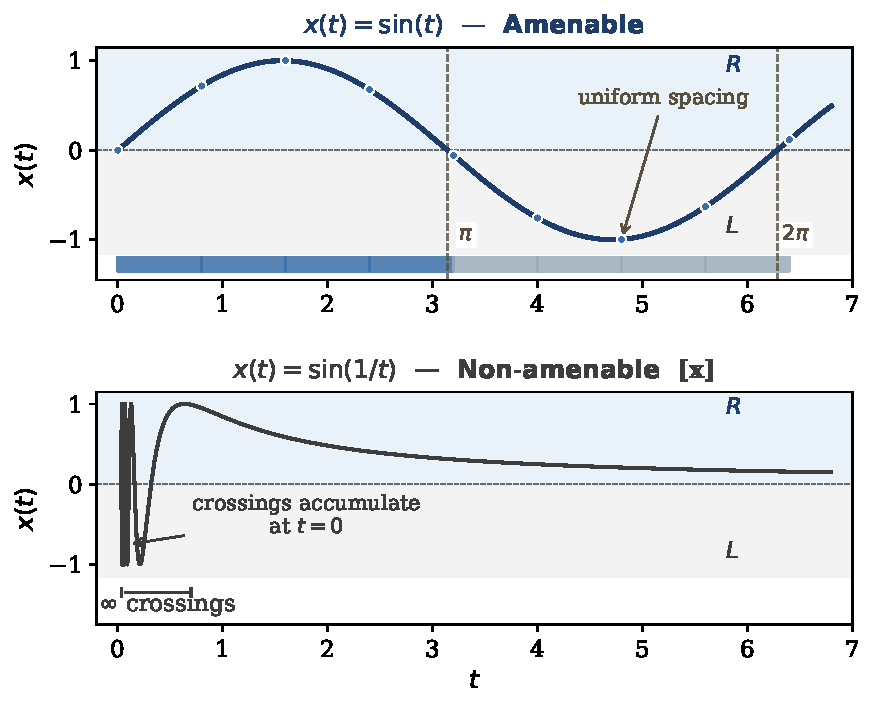
\includegraphics[width=0.78\textwidth]{figures/fig1_two_trajectories.pdf}
\caption{Two trajectories with identical range, smoothness class, and coarse-graining. $\sin(t)$ admits a stable symbolic description for $\Delta < \pi$; $\sin(1/t)$ does not for any fixed sampling interval near the origin. The relevant distinction is dwell time, not regularity.}
\label{fig:two-trajectories}
\end{figure}

This contrast brings the central question into focus. We are not asking whether continuous dynamics computes in every loose or semantic sense. We are asking when a sampled coarse-graining behaves like a genuine finite-state machine over a finite time window, and what physical resources are required to keep that description reliable for as long as it lasts. The answer has a structural part and a thermodynamic part. Structurally, a symbol must be readable by an observer, stable across the sampling interval, and predictive at the coarse-grained level. Thermodynamically, those properties are not simply given; near the boundary of failure they must be maintained against microscopic variability.

The argument proceeds in three steps. First, for sampled Markov microdynamics, we show that approximate lumpability makes the symbolic process close to a finite-state Markov chain in total variation, while decodability and stability say when that chain is readable and metastable. Second, we use that error budget to define a \emph{computation epoch}, the maximal window over which the symbolic description remains trustworthy at a chosen tolerance. Third, in a local perturbative two-cell model, we show that entropy production suppresses lumpability error as $\sqrt{\sigma}$ and therefore lengthens the achievable epoch, while the observer's Landauer cost supplies a second, unavoidable contribution to the work budget.

The emphasis is deliberate. Broader questions about geometric classification, optimisation over coarse-grainings, and stronger claims about macro-causal organisation are important, but they are not needed for the finite-horizon criterion developed here. By keeping the narrative tight, we can say more clearly what is proved, what is model-dependent, and where the thermodynamic content enters.

\paragraph{Relation to prior work.}
The structural side builds on classical lumpability for Markov chains \citep{kemeny1960,buchholz1994} and on modern metastability and Markov state model viewpoints \citep{deuflhard2005,schuette2013,husic2018}. Quantitative error bounds for Markov chain coarse-graining without scale separation have been developed by \citet{hilder2024}; finite-time bounds on the Markovian approximation error under lumping appear in \citet{andrieux2012}; \citet{geiger2025} surveys the information-theoretic landscape connecting coarse-graining to model reduction. The thermodynamic side draws on Landauer's principle and reversible computation \citep{landauer1961,bennett1982}, stochastic thermodynamics \citep{schnakenberg1976,seifert2012,wolpert2019}, and the broader programme connecting thermodynamic costs to computational structure \citep{wolpert2024arxiv}. Recent work by \citet{vandermeer2025} develops thermodynamic bounds and error-correction ideas for faulty coarse-graining with observation error, a setting complementary to the one studied here. What is added in the present paper is a direct, quantitative link between entropy production and lumpability error quality (Theorem~\ref{thm:dissipation}), together with the computation epoch as a finite-horizon construct that packages decodability, stability, and lumpability into a single error budget.

\section{Setup}\label{sec:setup}

We now formalise that intuition with the smallest amount of notation needed.

Let $X_t$ be a continuous-state process on a compact state space $\Xc \subset \R^d$. Fix a sampling interval $\Delta>0$ and write
\[
X_n := X_{n\Delta}, \qquad n=0,1,\ldots,N.
\]
Let $\Pi:\Xc \to [k] := \{1,\ldots,k\}$ be a coarse-graining map, and define the sampled symbolic process
\[
A_n := \Pi(X_n).
\]
Let $R_n$ denote the observer's physical record at time $n\Delta$. The problem is to determine when $(A_n)$ can be treated as a computational state sequence rather than as an arbitrary labelling of a restless continuum.

All Shannon entropies in this paper are measured in bits.

Three possible failures are immediate. A proposed symbol may be unreadable from the observer's record. It may change too quickly to support reliable state-to-state transitions. Or it may conceal unresolved microstructure that still matters for prediction. The next section turns those three failure modes into conditions.

\section{Readable, stable, predictive symbols}\label{sec:conditions}

We require three conditions on the triple $(X,\Pi,\Delta)$. They are not technical embellishments; they are the three ways a symbolic description can fail.

\begin{definition}[Decodability]\label{def:decodability}
The observer can recover the current symbol from the accessible record:
\[
H(A_n \mid R_n) \leq \varepsilon.
\]
By Fano's inequality, this yields a decoder $\hat{A}_n = \delta_n(R_n)$ with error probability
\[
\mathbb{P}(\hat{A}_n \neq A_n) \leq p_\varepsilon,
\]
where $p_\varepsilon \to 0$ as $\varepsilon \to 0$.
\end{definition}

Decodability is the minimal legibility condition. A symbol that cannot be read is not operationally available.

\begin{definition}[One-step stability]\label{def:stability}
The coarse-grained state persists across one sampling interval:
\[
\mathbb{P}(A_{n+1} \neq A_n) \leq \eta.
\]
\end{definition}

Stability makes room for causal use. If the symbol churns on the timescale at which it is sampled, it cannot function as a state.

\begin{definition}[Approximate lumpability]\label{def:lumpability}
For every symbol $i \in [k]$ and every step $n$,
\begin{equation}\label{eq:lumpability}
\sup_{\substack{x,y\,:\,\Pi(x)=\Pi(y)=i}}
\bigl|\Lc(A_{n+1}\mid X_n=x)-\Lc(A_{n+1}\mid X_n=y)\bigr|_{\TV}
\leq \lambda.
\end{equation}
\end{definition}

Approximate lumpability is the predictive condition. Once the coarse-grained state is known, residual microstate information should matter little for the next symbolic step.

\begin{remark}
The three conditions play different roles. Decodability makes symbols legible, stability makes them durable, and lumpability makes them informative about the future.
\end{remark}

\section{Markov approximation and computation epochs}\label{sec:markov}

Approximate lumpability is the structural ingredient that turns coarse states into an effective finite-state dynamics; decodability and stability then make that dynamics usable.

\begin{theorem}[Markov approximation]\label{thm:markov}
Let $X_0,\ldots,X_N$ be a sampled Markov chain on $\Xc$, whose transition law may depend on $n$, and let $A_n=\Pi(X_n)$. Suppose approximate lumpability holds for $n=0,\ldots,N-1$. Then there exists a time-inhomogeneous Markov chain $M_0,M_1,\ldots,M_N \in [k]$, with initial law $\Lc(M_0)=\Lc(A_0)$ and transition kernels
\[
K_n(j \mid i) := \mathbb{P}(A_{n+1}=j \mid A_n=i)
\]
such that
\begin{equation}\label{eq:markov-bound}
\bigl|\Lc(A_0,\ldots,A_N)-\Lc(M_0,\ldots,M_N)\bigr|_{\TV}
\leq N\lambda.
\end{equation}
If, in addition, decodability holds with decoders $\hat{A}_n=\delta_n(R_n)$ satisfying $\mathbb{P}(\hat{A}_n\neq A_n)\leq p_\varepsilon$ for each $n$, then
\begin{equation}\label{eq:decoded-bound}
\bigl|\Lc(\hat{A}_0,\ldots,\hat{A}_N)-\Lc(M_0,\ldots,M_N)\bigr|_{\TV}
\leq N\lambda + (N+1)p_\varepsilon.
\end{equation}
Finally, one-step stability implies metastability in the coarse chain:
\[
\mathbb{P}(M_{n+1}=M_n) \geq 1-\eta.
\]
\end{theorem}

The theorem is finite-horizon by design. The point is not that every continuous process can be reduced to a timeless automaton, but that over a controlled window the coarse-grained dynamics can behave like one to within an explicit error budget.

Real systems also drift. To compare a time window to a single machine, fix a starting time $n_0$ and suppose the symbolic kernels vary slowly:
\[
\sup_i \bigl|K_{n+1}(\cdot \mid i) - K_n(\cdot \mid i)\bigr|_{\TV} \leq \rho.
\]
A telescoping estimate then gives
\[
\sup_i \bigl|K_{n_0+r}(\cdot \mid i) - K_{n_0}(\cdot \mid i)\bigr|_{\TV} \leq r\rho,
\qquad r=0,\ldots,m-1,
\]
so over a window of length $m$ the discrepancy budget for the decoded symbolic path becomes
\[
m\lambda + (m+1)p_\varepsilon + \frac{\rho\,m(m-1)}{2}.
\]

\begin{definition}[Computation epoch]\label{def:epoch}
Given tolerance $\theta \in (0,1)$, the \emph{computation epoch} is
\begin{equation}\label{eq:epoch}
\Tc(\theta)
:=
\max\!\left\{
m\Delta :
m\lambda + (m+1)p_\varepsilon + \frac{\rho\,m(m-1)}{2} \leq \theta
\right\}.
\end{equation}
\end{definition}

This quantity packages the practical question. A system does not simply compute or fail to compute. Rather, at a chosen scale and accuracy, it supports a symbolic computation for a finite interval whose length is itself a physical observable. The two motivating trajectories make that distinction concrete.

\section{Dwell time in action: a worked comparison}\label{sec:example}

We return to the trajectories in \Eqref{eq:two-trajectories} under the binary partition $\Pi(x)=R$ for $x\geq 0$ and $L$ otherwise. Figure~\ref{fig:two-trajectories} already suggests the outcome geometrically; here we use it to isolate the role of dwell time. Because these are deterministic trajectories rather than sampled Markov microdynamics, the comparison is intended to illuminate the stability side of the framework rather than to instantiate Theorem~\ref{thm:markov} literally. To interpret the probabilistic statements below, let the initial sampling phase be distributed uniformly over the observation window.

\subsection{\texorpdfstring{$x(t)=\sin(t)$}{x(t)=sin(t)}}
Zero crossings occur at $t=n\pi$, separated by $\pi$. For $\Delta<\pi$, the trajectory has a uniform dwell time. If the initial phase is uniform over one period, the probability that the sign flips during one sample interval is exactly $\Delta/\pi$ for $0\leq \Delta \leq \pi$, so the induced binary sequence is stable on average when $\Delta$ is small. The point of the example is geometric: bounded crossing density creates a symbolic timescale.

\subsection{\texorpdfstring{$x(t)=\sin(1/t)$}{x(t)=sin(1/t)}}
Zero crossings occur at $t=1/(n\pi)$, with gaps that shrink to zero near the origin. No fixed $\Delta$ prevents arbitrarily rapid flipping in a sufficiently small neighbourhood of $t=0$. Hence there is no uniform dwell time and no observation window crossing the origin on which a fixed sampling interval yields a stable symbolic scale. The point is geometric rather than analytic: smoothness by itself does not protect symbolic dynamics when dwell times collapse.

\begin{table}[t]
\centering\small
\caption{Qualitative comparison of the geometric role played by the two trajectory examples.}
\label{tab:comparison}
\begin{tabular}{@{}lcc@{}}
\toprule
Property & $\sin(t)$ & $\sin(1/t)$ \\
\midrule
Uniform dwell time & Yes, with minimum gap $\pi$ & No, gaps accumulate at $0$ \\
Average one-step stability & Flip probability $\Delta/\pi$ for $\Delta<\pi$ & No uniform control near $t=0$ \\
Single symbolic timescale & Available & Breaks down near the origin \\
Role in the paper & Geometric prototype & Geometric obstruction \\
\bottomrule
\end{tabular}
\end{table}

The example also clarifies where thermodynamics enters. Dissipation can sharpen a noisy boundary or stabilise an already meaningful coarse state. It cannot create dwell time where the underlying trajectory provides none. Figure~\ref{fig:two-trajectories} therefore does more than motivate the paper: it marks the boundary between what thermodynamic maintenance may rescue and what geometry rules out from the start. With that boundary in view, we can now ask the physical question: when a coarse-grained symbolic dynamics is already geometrically meaningful, what keeps it coherent for long enough to be useful?

\section{Thermodynamic maintenance of symbolic dynamics}\label{sec:dissipation}

This is where dissipation enters. We ask where low lumpability error comes from physically. Consider a continuous-time Markov chain on a microstate space $\Omega$ with generator $Q$ and stationary distribution $\pi$. Its entropy production rate, following \citet{schnakenberg1976}, is
\begin{equation}\label{eq:entropy-prod}
\sigma(Q) =
\frac{1}{2}\sum_{x\neq y}
(\pi_x Q_{xy}-\pi_y Q_{yx})
\log\frac{\pi_x Q_{xy}}{\pi_y Q_{yx}}
\geq 0,
\end{equation}
with equality if and only if detailed balance holds.

Lumpability fails when microstates inside the same coarse cell have different one-step escape distributions. At equilibrium these differences are inherited from the landscape itself. A nonequilibrium perturbation can, in favourable directions, reduce that mismatch. The next theorem states a local version of this claim for a smooth perturbation family near detailed balance.

\begin{theorem}[Dissipation-lumpability inequality]\label{thm:dissipation}
Consider a smooth one-parameter family of generators $Q_\varepsilon$ on a four-state space $\{l_1,l_2,r_1,r_2\}$, with associated one-step kernels $P_\varepsilon = e^{\Delta Q_\varepsilon}$ and a two-cell coarse-graining $\Pi$ given by $L=\{l_1,l_2\}$ and $R=\{r_1,r_2\}$. Assume that $Q_0$ satisfies detailed balance, and write $\lambda_{\mathrm{eq}}(\Pi):=\lambda(P_0,\Pi)$. If the perturbation direction is aligned so that
\[
\frac{d}{d\varepsilon}\lambda(P_\varepsilon,\Pi)\Big|_{\varepsilon=0} = -c_0(\Pi) < 0,
\]
then
\begin{equation}\label{eq:dissipation-lumpability}
\lambda(P_\varepsilon,\Pi) = \lambda_{\mathrm{eq}}(\Pi) - c(\Pi)\sqrt{\sigma(Q_\varepsilon)} + O(\sigma(Q_\varepsilon)),
\end{equation}
where $c(\Pi)>0$. Equivalently, for any $0<c_-<c(\Pi)<c_+$ there exists $\sigma_0>0$ such that whenever $\sigma(Q_\varepsilon)\leq \sigma_0$,
\begin{equation}\label{eq:dissipation-two-sided}
\lambda_{\mathrm{eq}}(\Pi) - c_+\sqrt{\sigma(Q_\varepsilon)}
\leq
\lambda(P_\varepsilon,\Pi)
\leq
\lambda_{\mathrm{eq}}(\Pi) - c_-\sqrt{\sigma(Q_\varepsilon)}.
\end{equation}
\end{theorem}

The theorem should be read as a local maintenance law, not as a universal formula for every system. In the perturbative regime, entropy production buys predictive compression at the coarse-grained level. Along such a family, reducing $\lambda$ extends the computation epoch whenever the drift and decoding terms are held fixed. Figure~\ref{fig:dissipation} summarizes that logic in two panels: the left panel shows dissipation pressing down the lumpability error, while the right panel shows the same reduction reappearing as a longer interval of reliable symbolic dynamics.

\begin{figure}[t]
\centering
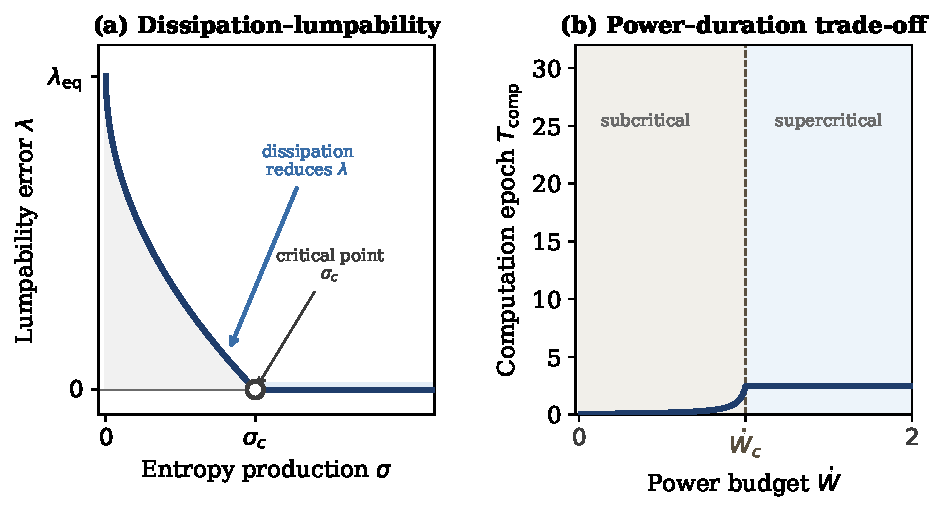
\includegraphics[width=0.82\textwidth]{figures/fig2_dissipation.pdf}
\caption{Left: in the perturbative regime, dissipation suppresses lumpability error as $\lambda_{\mathrm{eq}}-c\sqrt{\sigma}$. Right: through the epoch formula, reduced lumpability lengthens the reliable computation window. In the idealised limit of negligible decoding error and drift, the epoch grows without bound as $\lambda$ approaches zero.}
\label{fig:dissipation}
\end{figure}

\begin{corollary}[Power-duration trade-off]\label{cor:power}
Along a perturbation family satisfying Theorem~\ref{thm:dissipation}, if the substrate work rate satisfies $\dot{W}_{\mathrm{sub}} = k_BT\,\sigma(Q_\varepsilon)$ and the drift and decoding terms are fixed, then increasing the available power decreases $\lambda$ locally and therefore extends the achievable computation epoch.
\end{corollary}

The content of the corollary is modest but useful. It does not say that arbitrarily strong driving always helps, nor that the perturbative law continues unchanged far from equilibrium. It says that within the controlled regime of the theorem, a longer reliable symbolic computation window requires thermodynamic maintenance. Read together, the two panels of Figure~\ref{fig:dissipation} give the paper's thermodynamic middle act: dissipation first reorganizes the coarse dynamics, and only then appears as extra duration at the symbolic level. Yet the substrate is only half the story: a computation must also be read.

\section{Observer cost and total work}\label{sec:observer}

The symbolic dynamics is only operational if an observer can record it. That requirement has its own physical cost. By Landauer's principle \citep{landauer1961,bennett1982}, resetting a memory register incurs work at least $k_BT\ln 2$ per erased bit.

Decodability already forces the record to contain information about the current symbol. Indeed,
\[
I(A_n;R_n) = H(A_n)-H(A_n\mid R_n) \geq H(A_n)-\varepsilon,
\]
and since $I(A_n;R_n)\leq H(R_n)$, any record from which the current symbol can be decoded with conditional entropy at most $\varepsilon$ must satisfy
\[
H(R_n)\geq H(A_n)-\varepsilon.
\]
If that record is reset after each sampling step, erasing it costs at least $k_BT\ln 2 \cdot H(R_n)$.

Let $m = \Tc/\Delta$ denote the number of sampling steps in a target epoch. Suppose the total tolerance budget $\theta$ is split into three non-negative parts
\[
\theta = \theta_{\mathrm{lump}} + \theta_{\mathrm{dec}} + \theta_{\mathrm{drift}},
\]
corresponding to lumpability, decoding, and temporal drift. If
\[
m\lambda \leq \theta_{\mathrm{lump}}, \qquad
(m+1)p_\varepsilon \leq \theta_{\mathrm{dec}}, \qquad
\frac{\rho\,m(m-1)}{2} \leq \theta_{\mathrm{drift}},
\]
then the epoch constraint in \Eqref{eq:epoch} is satisfied.

\begin{proposition}[Lower bound on total work]\label{prop:cost}
Fix a target epoch $\Tc=m\Delta$ and a tolerance split with $\theta_{\mathrm{lump}}>0$. Assume the substrate lies in the local perturbative regime of Theorem~\ref{thm:dissipation}, and choose a constant $c_+>c(\Pi)$ for which the lower bound in \Eqref{eq:dissipation-two-sided} holds throughout the relevant range. Then the substrate work required to meet the lumpability budget obeys
\begin{equation}\label{eq:substrate-bound}
W_{\mathrm{sub}}(\Tc)
\geq
k_BT\,\Tc\,
\left(
\frac{\bigl(\lambda_{\mathrm{eq}}-\theta_{\mathrm{lump}}/m\bigr)_+}{c_+}
\right)^{\!2},
\end{equation}
where $(u)_+ := \max\{u,0\}$. If, moreover, the observer resets the record after each of the $m+1$ samples in the epoch, then the recording cost satisfies
\begin{equation}\label{eq:observer-bound}
W_{\mathrm{obs}}(\Tc)
\geq
k_BT\ln 2
\sum_{n=0}^{m}\bigl(H(A_n)-\varepsilon\bigr)_+.
\end{equation}
Hence
\begin{equation}\label{eq:total-bound}
W_{\mathrm{total}}(\Tc) \geq W_{\mathrm{sub}}(\Tc) + W_{\mathrm{obs}}(\Tc).
\end{equation}
\end{proposition}

The proposition separates two expenses that are often conflated. One pays to make the coarse-grained dynamics predictive; the other pays to read and store the resulting symbols. Computation, in this sense, is a property of the coupled system-observer pair. The narrative of the paper can now be stated cleanly: geometry makes symbolic persistence possible, probability theory turns that persistence into an effective finite-state model, and thermodynamics determines how expensively the model can be maintained and read.

\section{Discussion}\label{sec:discussion}

Viewed from a distance, the paper tells a simple story. A continuous process supports a finite-state computation over a finite window only when its coarse-graining is readable, stable on the sampling timescale, and approximately lumpable. Those three properties yield a Markov approximation and therefore a well-defined computation epoch. Maintaining that epoch is not free: in the perturbative model studied here, dissipation reduces lumpability error, while observation adds an independent recording cost.

That narrower claim is useful precisely because it avoids saying too much. We do not prove that every meaningful computation in continuous media must take the form analysed here. We do not classify all trajectories or optimise over all possible partitions. We do not derive a universal non-equilibrium scaling law beyond the local two-cell regime. What we do obtain is a clean finite-horizon criterion and a thermodynamic interpretation of why reliable symbolic dynamics is special rather than generic.

Several extensions are natural. The first is to move beyond the perturbative two-cell setting and ask whether a similar dissipation-lumpability relation persists when metastable coarse-grainings shape the dynamics in the small-noise regime \citep{freidlin1984}. A second is to optimise the partition itself under a joint budget on dissipation and decoding cost. A third is empirical: the framework suggests concrete diagnostics for physical substrates, namely measured dwell times, inferred coarse transition kernels, and the energy required to stabilise and read them. Unifying these perspectives with the quantitative coarse-graining bounds of \citep{hilder2024,andrieux2012} and the thermodynamic analysis of faulty coarse-graining with observation error in \citep{vandermeer2025} beyond the perturbative regime is a natural direction for future work.

\paragraph{Interactive materials.}
Code and interactive figures are available at \url{https://jonland82.github.io/continuous-computation/}.

\begin{appendices}

\section{Proof of the Markov approximation theorem}\label{app:markov}

We prove Theorem~\ref{thm:markov}. Let
\[
K_n(j \mid i) := \mathbb{P}(A_{n+1}=j \mid A_n=i).
\]
Define $M_0,\ldots,M_N$ by $\Lc(M_0)=\Lc(A_0)$ and transition kernels $K_n$.

\textbf{Step 1: one-step Markovization.}
Because $X_n$ is Markov, conditioning on the full symbolic past affects the next symbol only through the conditional distribution of $X_n$. For every history $(a_0,\ldots,a_n)$ with $a_n=i$,
\[
\Lc(A_{n+1}\mid A_0=a_0,\ldots,A_n=i)
=
\int_{\Pi^{-1}(i)} \Lc(A_{n+1}\mid X_n=x)\,d\mu_{a_0,\ldots,a_n}(x),
\]
for a probability measure $\mu_{a_0,\ldots,a_n}$ supported on the cell $\Pi^{-1}(i)$. The kernel $K_n(\cdot \mid i)=\Lc(A_{n+1}\mid A_n=i)$ is another mixture of the same family of measures over the same cell. By approximate lumpability, any two such mixtures differ by at most $\lambda$ in total variation. Hence
\[
\bigl|\Lc(A_{n+1}\mid A_0,\ldots,A_n)-K_n(\cdot \mid A_n)\bigr|_{\TV}
\leq \lambda
\]
almost surely.

\textbf{Step 2: telescoping along the path.}
Compare the path laws of $(A_0,\ldots,A_N)$ and $(M_0,\ldots,M_N)$ by coupling them step by step. The initial laws agree, and at each stage the one-step conditional discrepancy is at most $\lambda$. A standard telescoping/coupling argument for total variation on path space then gives (see, e.g., \citep{levin2017})
\[
\bigl|\Lc(A_0,\ldots,A_N)-\Lc(M_0,\ldots,M_N)\bigr|_{\TV}
\leq N\lambda.
\]

\textbf{Step 3: decoded path.}
Let $E:=\{\exists\,n\in\{0,\ldots,N\}: \hat{A}_n\neq A_n\}$. By the union bound,
\[
\mathbb{P}(E)\leq (N+1)p_\varepsilon.
\]
Couple the decoded path to the true symbolic path on the same probability space. Then
\[
\bigl|\Lc(\hat{A}_0,\ldots,\hat{A}_N)-\Lc(A_0,\ldots,A_N)\bigr|_{\TV}
\leq \mathbb{P}(E)
\leq (N+1)p_\varepsilon.
\]
Combining this with Step 2 proves \Eqref{eq:decoded-bound}.

\textbf{Step 4: metastability.}
By construction, $M_n$ and $A_n$ have the same one-time marginals for every $n$. Therefore
\[
\mathbb{P}(M_{n+1}=M_n)
=
\sum_i \mathbb{P}(A_n=i)K_n(i\mid i)
=
\mathbb{P}(A_{n+1}=A_n)
\geq 1-\eta.
\]
This is the stated metastability bound. \qed

\section{Proof of the dissipation-lumpability inequality}\label{app:dissipation}

We prove Theorem~\ref{thm:dissipation} for a smooth family of generators $Q_\varepsilon$ on the four-state, two-cell model. Write the two coarse cells as
\[
L=\{l_1,l_2\}, \qquad R=\{r_1,r_2\}.
\]
Let $P_\varepsilon=e^{\Delta Q_\varepsilon}$ and define the lumpability error for the transition $L \to R$ by
\[
\lambda(\varepsilon) = |e_1(\varepsilon)-e_2(\varepsilon)|,
\qquad
e_i(\varepsilon) := \sum_j (P_\varepsilon)_{l_i r_j}.
\]

\textbf{Equilibrium baseline.}
At $\varepsilon=0$, the generator $Q_0$ satisfies detailed balance. Set $\lambda_{\mathrm{eq}}:=\lambda(0)$.

\textbf{Perturbation.}
Because $\varepsilon \mapsto P_\varepsilon$ is smooth, so is $\lambda(\varepsilon)$. By assumption, the perturbation direction is aligned so that $\lambda'(0)=-c_0<0$. Therefore
\[
\lambda(\varepsilon)
=
\lambda_{\mathrm{eq}} - c_0\,\varepsilon + O(\varepsilon^2).
\]

\textbf{Connecting to entropy production.}
Near detailed balance, entropy production has the expansion
\[
\sigma(Q_\varepsilon) = \varepsilon^2 \sigma_2 + O(\varepsilon^3),
\qquad \sigma_2>0.
\]
Hence
\[
\varepsilon = \frac{1}{\sqrt{\sigma_2}}\sqrt{\sigma(Q_\varepsilon)} + O(\sigma(Q_\varepsilon)),
\]
and substitution yields
\[
\lambda(P_\varepsilon,\Pi)
=
\lambda_{\mathrm{eq}}(\Pi) - c(\Pi)\sqrt{\sigma(Q_\varepsilon)} + O(\sigma(Q_\varepsilon)),
\qquad
c(\Pi):=\frac{c_0}{\sqrt{\sigma_2}}.
\]
This proves \Eqref{eq:dissipation-lumpability}.

\textbf{Two-sided local bound.}
Fix $0<c_-<c(\Pi)<c_+$. Since the remainder is $O(\sigma)$ and $\sqrt{\sigma}$ dominates $\sigma$ as $\sigma\to 0$, there exists $\sigma_0>0$ such that whenever $\sigma(Q_\varepsilon)\leq \sigma_0$,
\[
\lambda_{\mathrm{eq}}(\Pi) - c_+\sqrt{\sigma(Q_\varepsilon)}
\leq
\lambda(P_\varepsilon,\Pi)
\leq
\lambda_{\mathrm{eq}}(\Pi) - c_-\sqrt{\sigma(Q_\varepsilon)}.
\]
This is \Eqref{eq:dissipation-two-sided}. \qed

\section{Derivation of the work bound}\label{app:cost}

Let $\Tc=m\Delta$ and suppose the tolerance budget is split as in Section~\ref{sec:observer}. To satisfy the lumpability budget it is sufficient that
\[
\lambda \leq \frac{\theta_{\mathrm{lump}}}{m}.
\]
In the local perturbative regime, choose $c_+>c(\Pi)$ so that
\[
\lambda \geq \lambda_{\mathrm{eq}} - c_+\sqrt{\sigma}.
\]
Combined with the lumpability budget $\lambda \leq \theta_{\mathrm{lump}}/m$, the lower bound gives
\[
\lambda_{\mathrm{eq}} - c_+\sqrt{\sigma}
\leq
\frac{\theta_{\mathrm{lump}}}{m},
\]
and hence
\[
\sqrt{\sigma}
\geq
\frac{\bigl(\lambda_{\mathrm{eq}}-\theta_{\mathrm{lump}}/m\bigr)_+}{c_+}.
\]
Squaring both sides gives
\[
\sigma
\geq
\left(
\frac{\bigl(\lambda_{\mathrm{eq}}-\theta_{\mathrm{lump}}/m\bigr)_+}{c_+}
\right)^2.
\]
Since $W_{\mathrm{sub}} = k_BT\,\Tc\,\sigma$, this yields \Eqref{eq:substrate-bound}.

For the observer, decodability gives $H(R_n)\geq H(A_n)-\varepsilon$ for every $n$. Erasing the record at step $n$ therefore costs at least
\[
k_BT\ln 2 \cdot \bigl(H(A_n)-\varepsilon\bigr)_+.
\]
Summing over the $m+1$ sampled records yields \Eqref{eq:observer-bound}. Adding the two contributions yields \Eqref{eq:total-bound}. \qed

\end{appendices}

\bibliographystyle{plainnat}
\begin{thebibliography}{16}

\bibitem[Kemeny and Snell(1960)]{kemeny1960}
J.~G. Kemeny and J.~L. Snell.
\emph{Finite Markov Chains}.
Van Nostrand, 1960.

\bibitem[Buchholz(1994)]{buchholz1994}
P.~Buchholz.
Exact and ordinary lumpability in finite Markov chains.
\emph{J. Appl. Probab.}, 31(1):59--75, 1994.

\bibitem[Deuflhard and Weber(2005)]{deuflhard2005}
P.~Deuflhard and M.~Weber.
Robust Perron cluster analysis in conformation dynamics.
\emph{Linear Algebra Appl.}, 398:161--184, 2005.

\bibitem[Sch\"utte and Sarich(2013)]{schuette2013}
C.~Sch\"utte and M.~Sarich.
\emph{Metastability and Markov State Models in Molecular Dynamics}.
American Mathematical Society, 2013.

\bibitem[Husic and Pande(2018)]{husic2018}
B.~E. Husic and V.~S. Pande.
Markov state models: From an art to a science.
\emph{J. Am. Chem. Soc.}, 140(7):2386--2396, 2018.

\bibitem[Landauer(1961)]{landauer1961}
R.~Landauer.
Irreversibility and heat generation in the computing process.
\emph{IBM J. Res. Dev.}, 5:183--191, 1961.

\bibitem[Bennett(1982)]{bennett1982}
C.~H. Bennett.
The thermodynamics of computation: a review.
\emph{Int. J. Theor. Phys.}, 21:905--940, 1982.

\bibitem[Schnakenberg(1976)]{schnakenberg1976}
J.~Schnakenberg.
Network theory of microscopic and macroscopic behavior of master equation systems.
\emph{Rev. Mod. Phys.}, 48:571--585, 1976.

\bibitem[Seifert(2012)]{seifert2012}
U.~Seifert.
Stochastic thermodynamics, fluctuation theorems and molecular machines.
\emph{Rep. Prog. Phys.}, 75(12):126001, 2012.

\bibitem[Wolpert(2019)]{wolpert2019}
D.~H. Wolpert.
The stochastic thermodynamics of computation.
\emph{J. Phys. A: Math. Theor.}, 52(19):193001, 2019.

\bibitem[Freidlin and Wentzell(1984)]{freidlin1984}
M.~I. Freidlin and A.~D. Wentzell.
\emph{Random Perturbations of Dynamical Systems}.
Springer, 1984.

\bibitem[Levin and Peres(2017)]{levin2017}
D.~A. Levin and Y.~Peres.
\emph{Markov Chains and Mixing Times}.
American Mathematical Society, 2nd edition, 2017.

\bibitem[Hilder and Sharma(2024)]{hilder2024}
B.~Hilder and U.~Sharma.
Quantitative coarse-graining of Markov chains.
\emph{SIAM J. Math. Anal.}, 56(1):913--954, 2024.

\bibitem[Andrieux(2012)]{andrieux2012}
D.~Andrieux.
Bounding the coarse graining error in hidden Markov dynamics.
\emph{Appl. Math. Lett.}, 25(11):1734--1739, 2012.

\bibitem[Geiger(2026)]{geiger2025}
B.~C. Geiger.
Information-theoretic reduction of Markov chains.
\emph{Computer Science Review}, 59:100802, 2026.
\newblock DOI: 10.1016/j.cosrev.2025.100802.

\bibitem[van der Meer and Saito(2025)]{vandermeer2025}
J.~van der Meer and K.~Saito.
Thermodynamic bounds and error correction for faulty coarse graining.
\emph{Phys. Rev. Research}, 7(4):043260, 2025.
\newblock DOI: 10.1103/PhysRevResearch.7.043260.

\bibitem[Wolpert et~al.(2024)]{wolpert2024arxiv}
D.~H. Wolpert et~al.
Is stochastic thermodynamics the key to understanding the energy costs of computation?
\emph{Proc. Natl. Acad. Sci. U.S.A.}, 121(45):e2321112121, 2024.
\newblock DOI: 10.1073/pnas.2321112121.

\end{thebibliography}

\end{document}
